\documentclass{article}

\usepackage{subcaption}
\usepackage[labelformat=parens,labelsep=quad,skip=3pt]{caption}
\usepackage{graphicx}
\usepackage{geometry}

%\geometry{top=0.1in, left=0.1in, right=0.1in, bottom=0.1in}

\usepackage{array}
\usepackage{makecell}
\usepackage{tabularx}
\usepackage[dvipsnames]{xcolor}
\usepackage{amssymb}
\renewcommand{\tabularxcolumn}[1]{m{#1}}

%\pdfpageheight=5in
%\pdfpagewidth=7.2in

\begin{document}
	\section{Single Subject Estimates}
	\begin{tabularx}{7in}{|m{1em}|X|X|X|X|}
		\hline
		& \multicolumn{1}{c|}{Visual Cue} & \multicolumn{1}{c|}{Tongue} & \multicolumn{1}{c|}{Right Foot} & \multicolumn{1}{c|}{Right Hand} \\ \hline
		\rotatebox{90}{\textbf{Bayesian GLM}}& 
		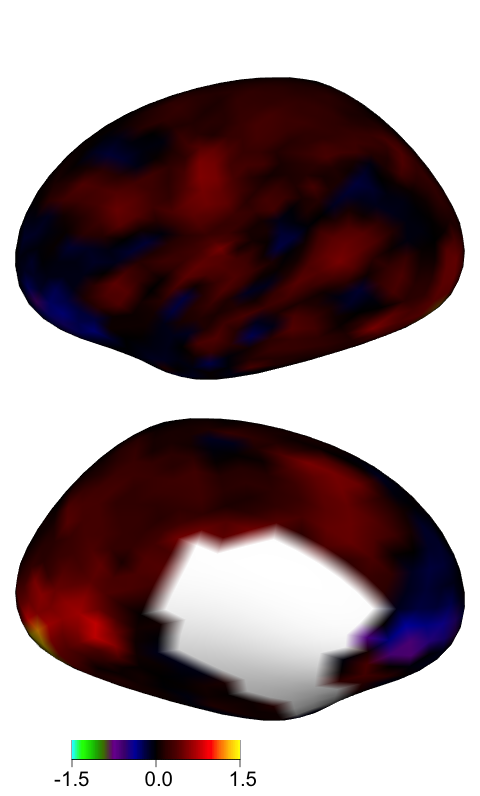
\includegraphics[width=1.5in]{plots/601_single_subject_Bayes_visual_cue.png} &
		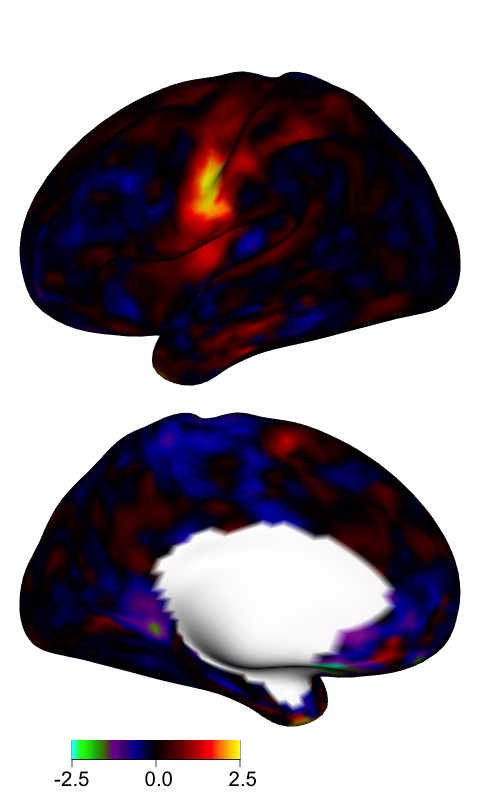
\includegraphics[width=1.5in]{plots/601_single_subject_Bayes_tongue.png} &
		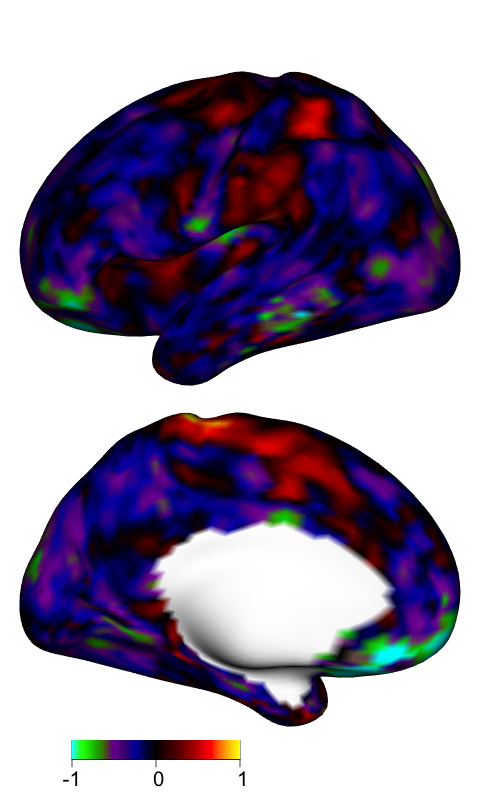
\includegraphics[width=1.5in]{plots/601_single_subject_Bayes_right_foot.png} &
		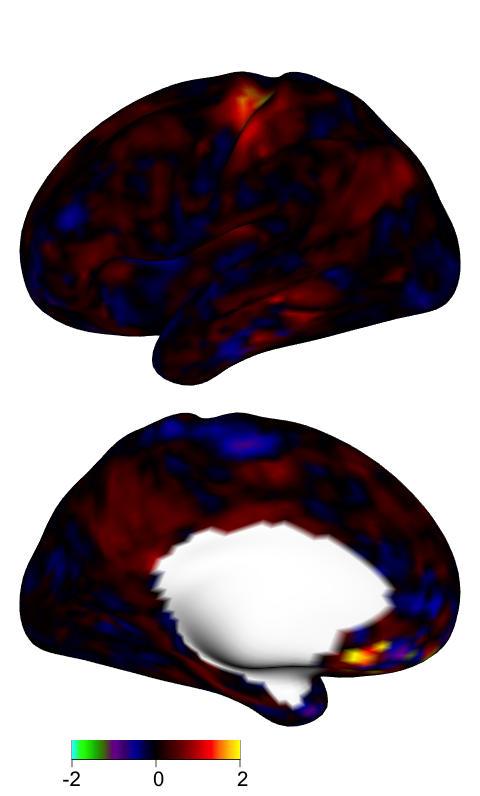
\includegraphics[width=1.5in]{plots/601_single_subject_Bayes_right_hand.png} \\ \hline
		\rotatebox{90}{\textbf{Classical GLM}} & 
		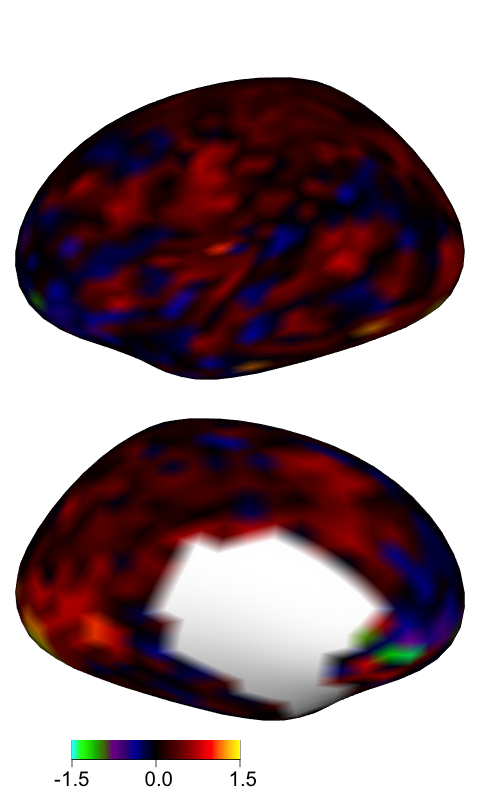
\includegraphics[width=1.5in]{plots/601_single_subject_classical_visual_cue.png} &
		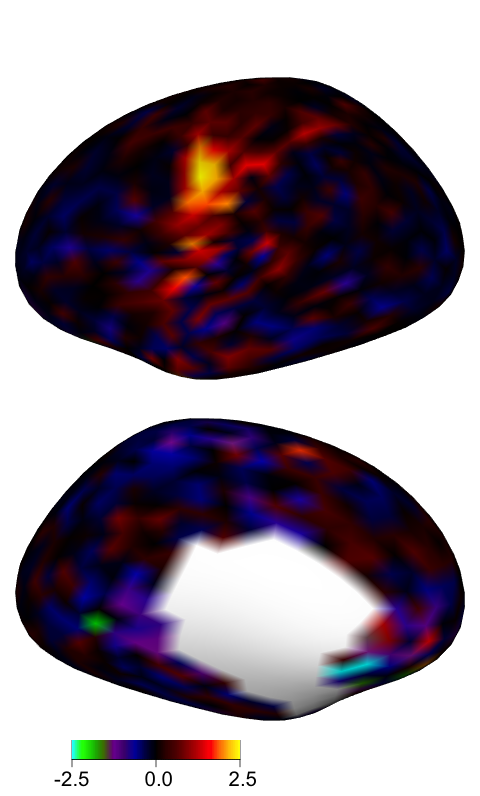
\includegraphics[width=1.5in]{plots/601_single_subject_classical_tongue.png} &
		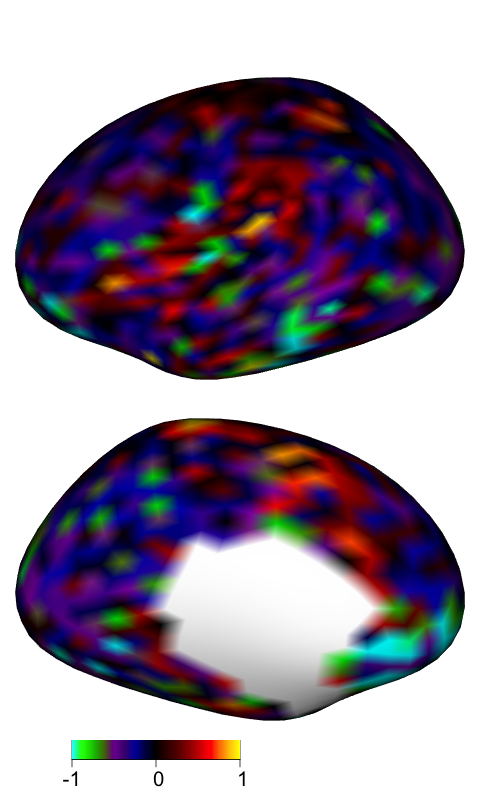
\includegraphics[width=1.5in]{plots/601_single_subject_classical_right_foot.png} &
		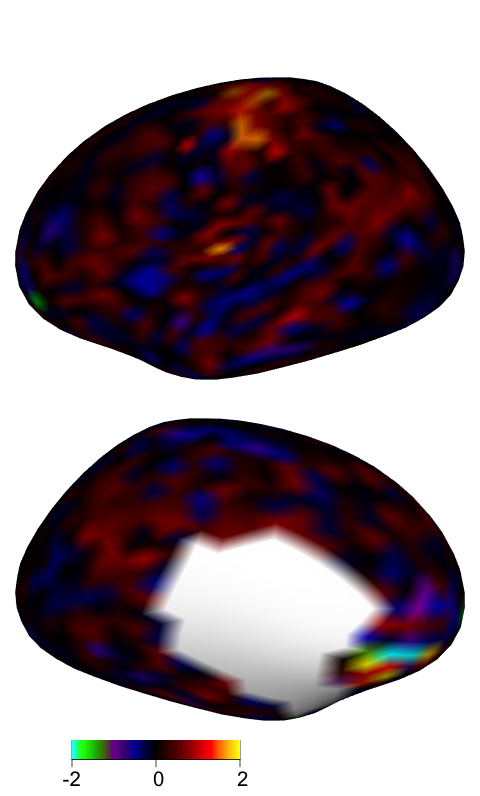
\includegraphics[width=1.5in]{plots/601_single_subject_classical_right_hand.png} \\ \hline
	\end{tabularx}
	
	\newpage
	
	\section{Group Estimates}
	\begin{tabularx}{7in}{|m{1em}|X|X|X|X|}
		\hline
		& \multicolumn{1}{c|}{Visual Cue} & \multicolumn{1}{c|}{Tongue} & \multicolumn{1}{c|}{Right Foot} & \multicolumn{1}{c|}{Right Hand} \\ \hline
		\rotatebox{90}{\textbf{Bayesian GLM}}& 
		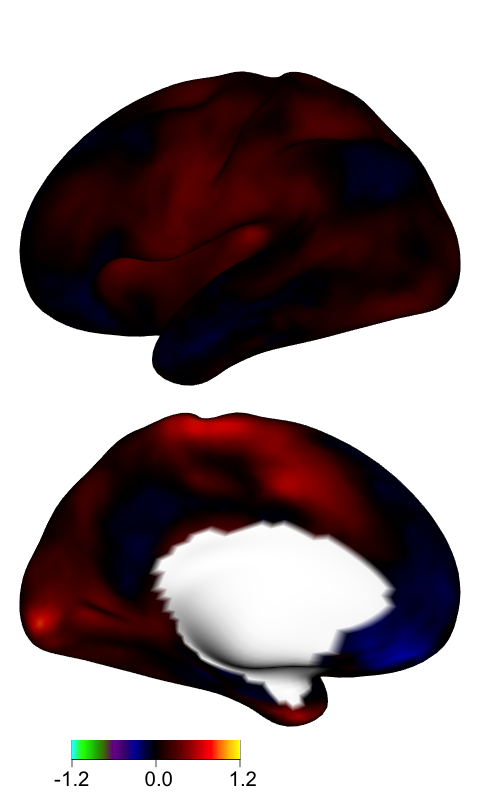
\includegraphics[width=1.5in]{plots/601_group_Bayes_visual_cue.png} &
		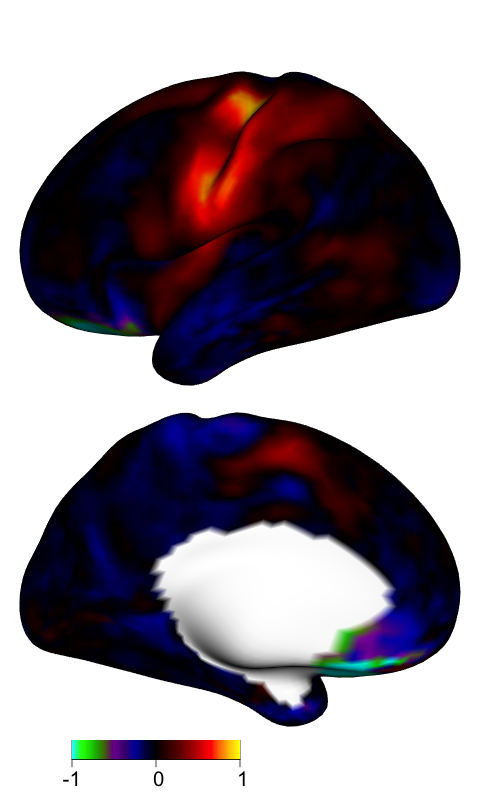
\includegraphics[width=1.5in]{plots/601_group_Bayes_tongue.png} &
		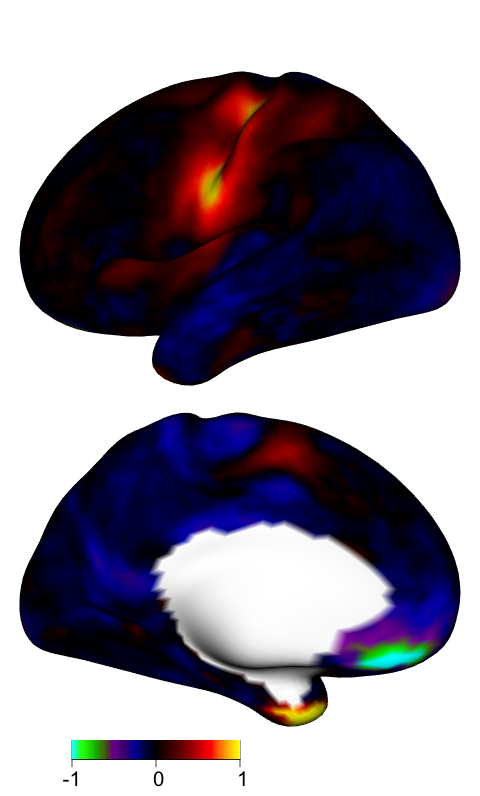
\includegraphics[width=1.5in]{plots/601_group_Bayes_right_foot.png} &
		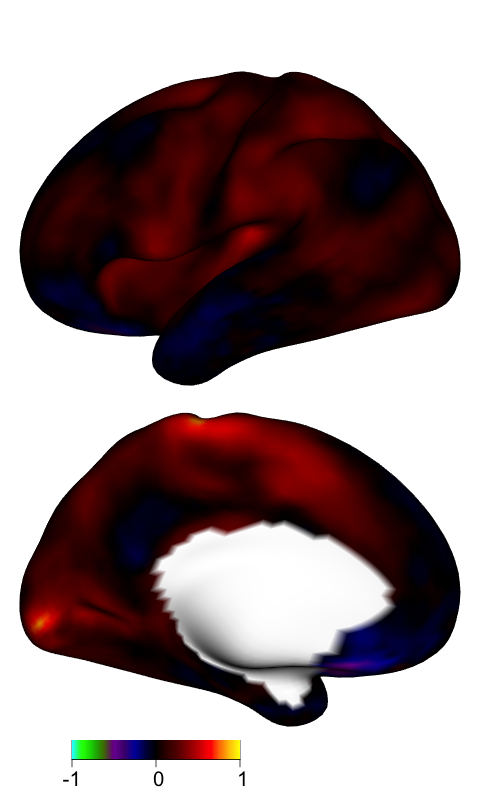
\includegraphics[width=1.5in]{plots/601_group_Bayes_right_hand.png} \\ \hline
		\rotatebox{90}{\textbf{Classical GLM}} & 
		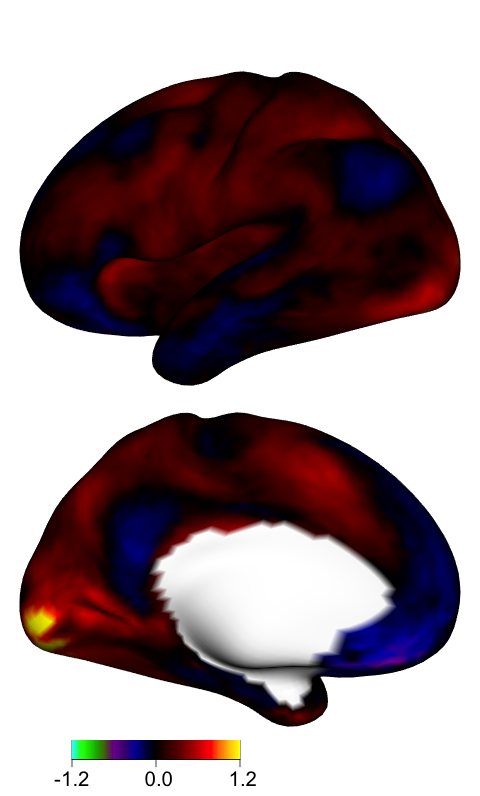
\includegraphics[width=1.5in]{plots/601_group_classical_visual_cue.png} &
		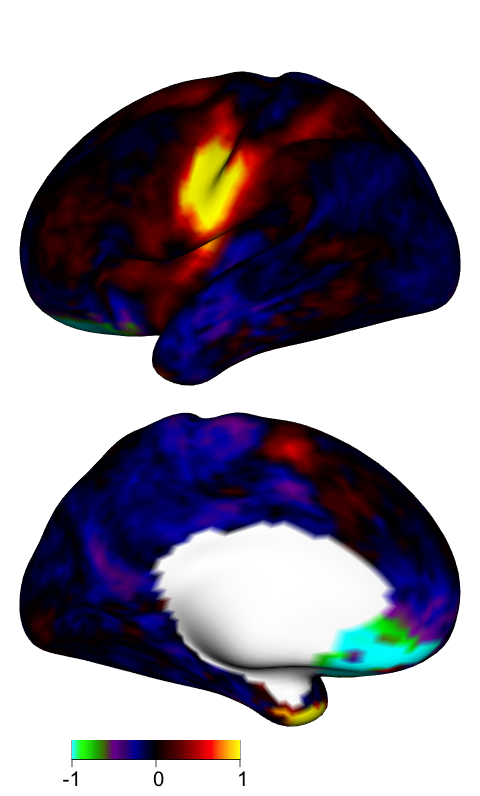
\includegraphics[width=1.5in]{plots/601_group_classical_tongue.png} &
		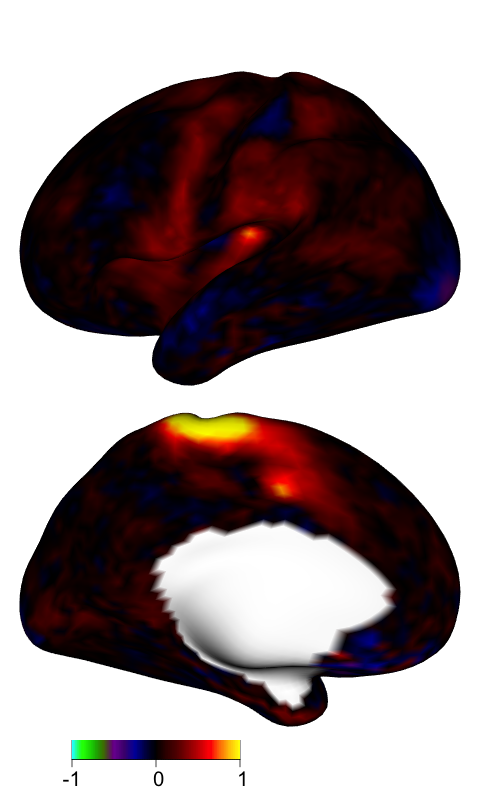
\includegraphics[width=1.5in]{plots/601_group_classical_right_foot.png} &
		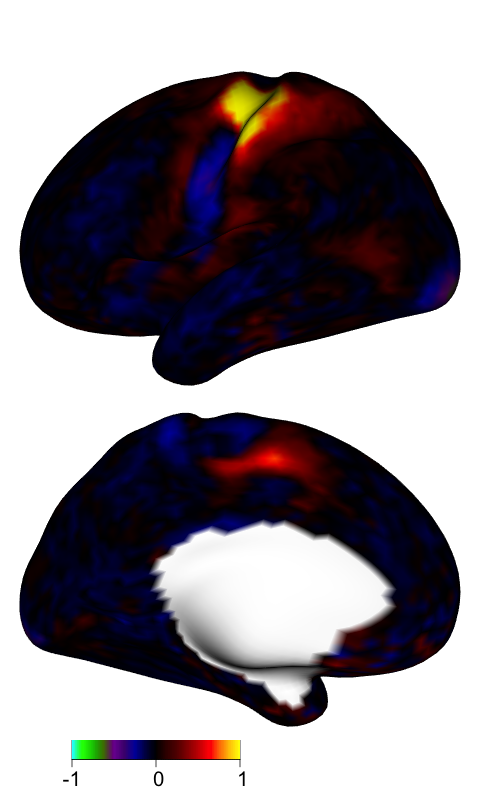
\includegraphics[width=1.5in]{plots/601_group_classical_right_hand.png} \\ \hline
	\end{tabularx}

	\newpage

	\section{Activation}
	\begin{tabularx}{7in}{|m{1em}|X|X|X|X|}
		\hline
		& \multicolumn{1}{c|}{Visual Cue} & \multicolumn{1}{c|}{Tongue} & \multicolumn{1}{c|}{Right Foot} & \multicolumn{1}{c|}{Right Hand} \\ \hline
		\rotatebox{90}{\textbf{Bayesian GLM}}& 
		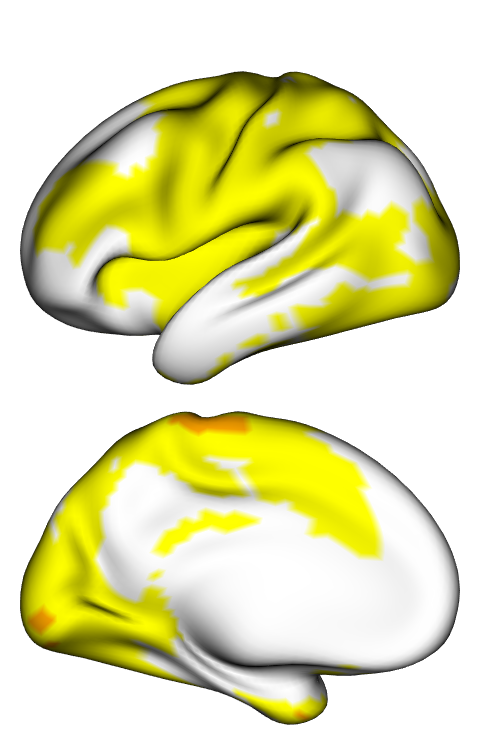
\includegraphics[width=1.5in]{plots/603_visual_cue_activation_map.png} &
		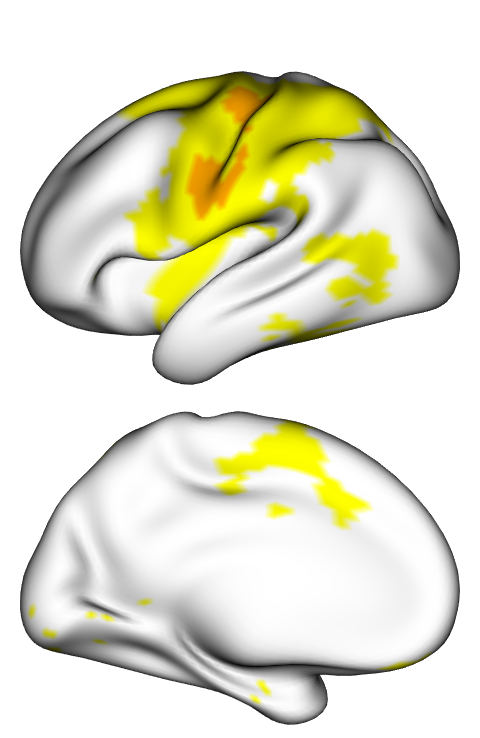
\includegraphics[width=1.5in]{plots/603_tongue_activation_map.png} &
		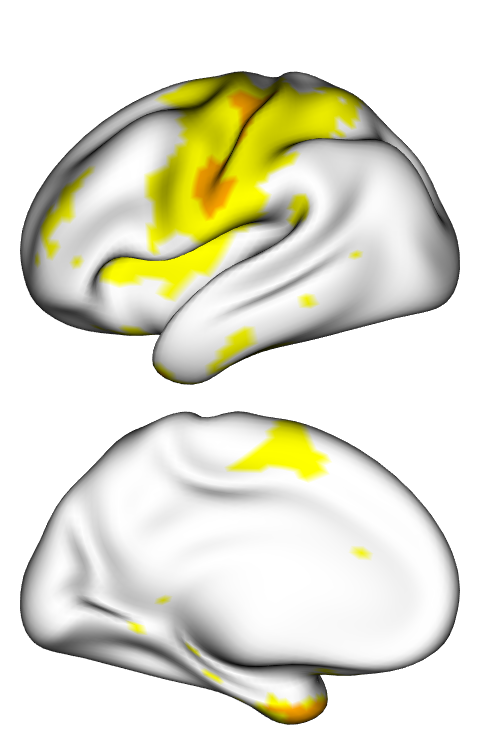
\includegraphics[width=1.5in]{plots/603_foot_activation_map.png} &
		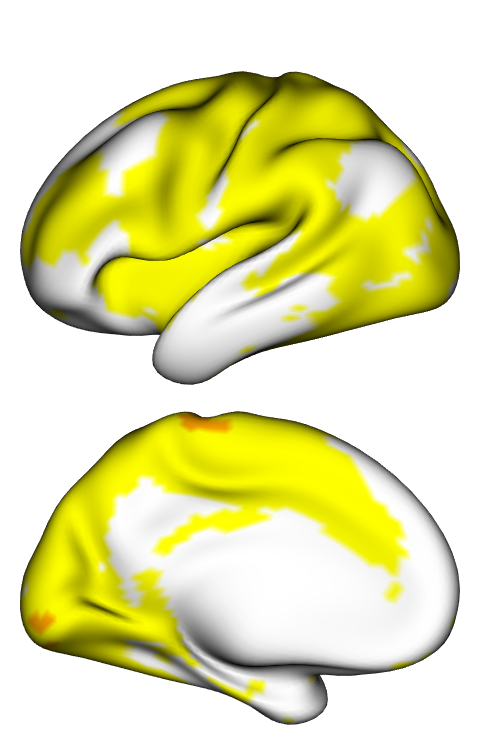
\includegraphics[width=1.5in]{plots/603_hand_activation_map.png} \\ \hline
		\multicolumn{2}{c}{} & \multicolumn{2}{c}{$\gamma = $ \textcolor{yellow}{$\blacksquare$} $0\%$ \textcolor{orange}{$\blacksquare$} $0.5\%$ } & \multicolumn{1}{c}{} \\ \hline
		\rotatebox{90}{\textbf{Classical GLM}} & 
		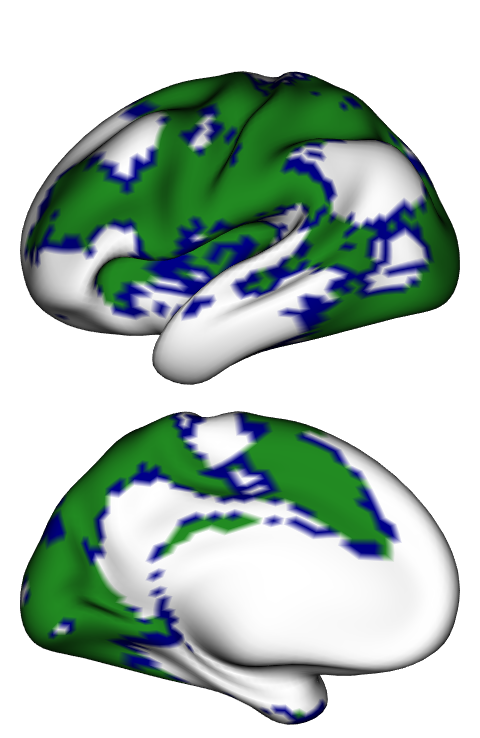
\includegraphics[width=1.5in]{plots/604_visual_cue_classical_activation_map.png} &
		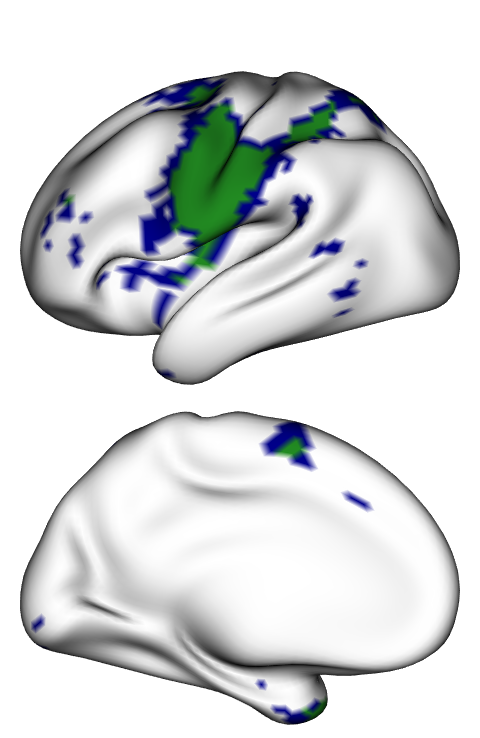
\includegraphics[width=1.5in]{plots/604_tongue_classical_activation_map.png} &
		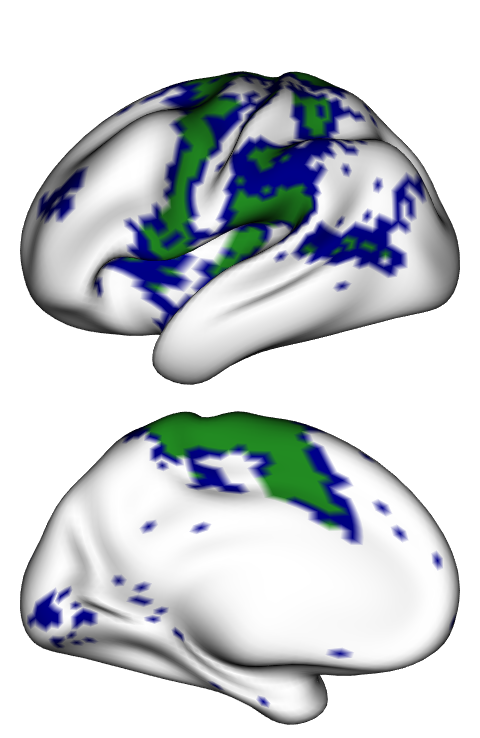
\includegraphics[width=1.5in]{plots/604_foot_classical_activation_map.png} &
		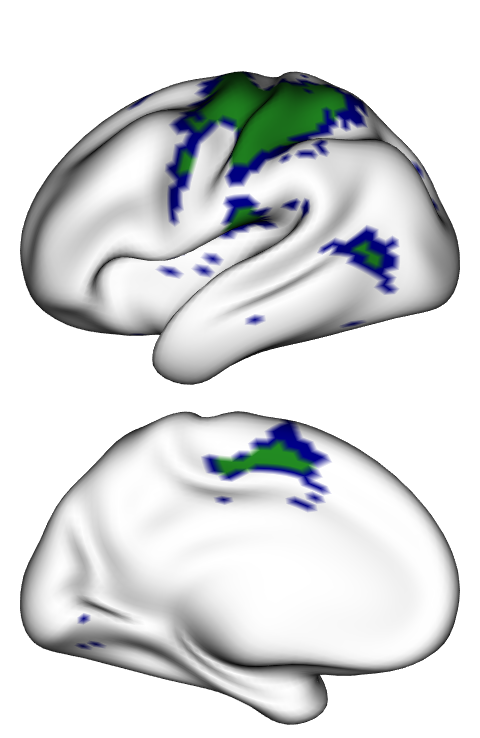
\includegraphics[width=1.5in]{plots/604_hand_classical_activation_map.png} \\ \hline
		\multicolumn{2}{c}{} & \multicolumn{2}{c}{\textcolor{MidnightBlue}{$\blacksquare$} FDR \textcolor{OliveGreen}{$\blacksquare$} FWER } & \multicolumn{1}{c}{} \\
	\end{tabularx}	

%	\newpage
%	
%	\pagestyle{empty}
%
%	\begin{figure}
%		\begin{subfigure}{\textwidth}
%			\begin{tabularx}{\textwidth}{|m{1em}|X|X|X|X|}
%				\multicolumn{1}{c}{} & \multicolumn{1}{c}{\textbf{Visual Cue}} & \multicolumn{1}{c}{\textbf{Tongue}} & \multicolumn{1}{c}{\textbf{Right Foot}} & \multicolumn{1}{c}{\textbf{Right Hand}} \\ \hline
%				\rotatebox{90}{\textbf{Bayesian GLM}}& 
%				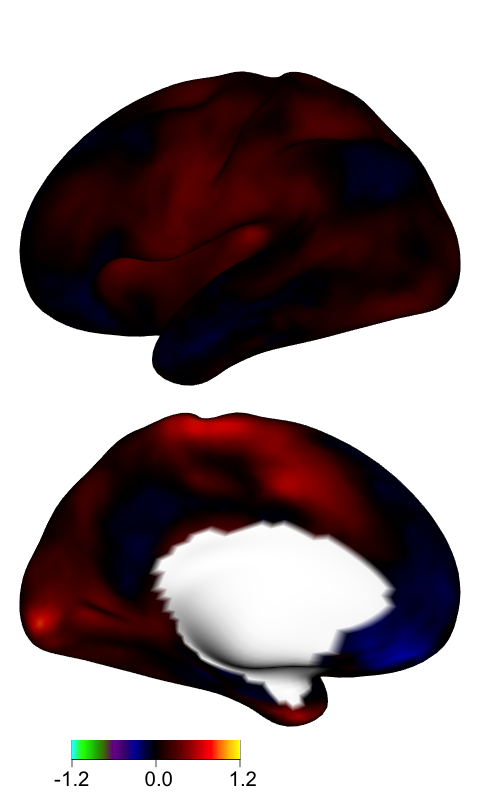
\includegraphics[width=0.2\textwidth]{plots/601_group_Bayes_visual_cue.png} &
%				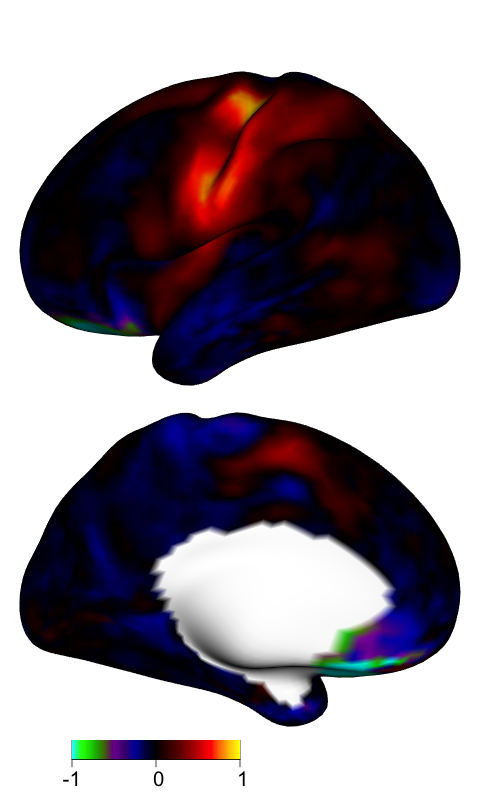
\includegraphics[width=0.2\textwidth]{plots/601_group_Bayes_tongue.png} &
%				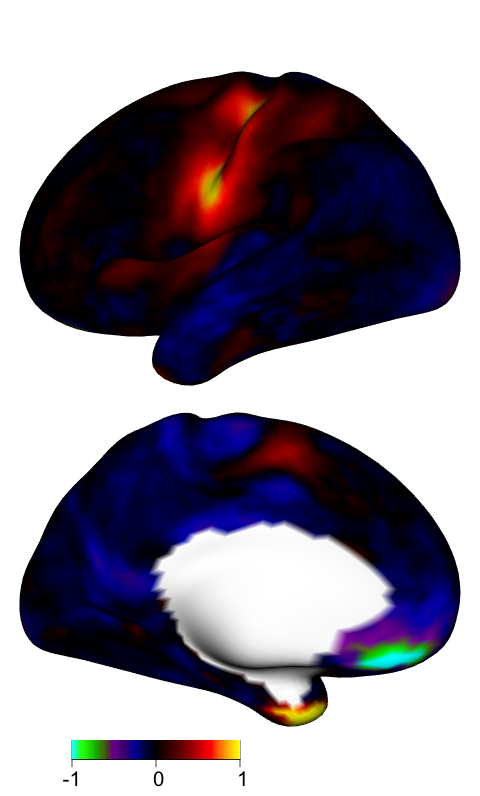
\includegraphics[width=0.2\textwidth]{plots/601_group_Bayes_right_foot.png} &
%				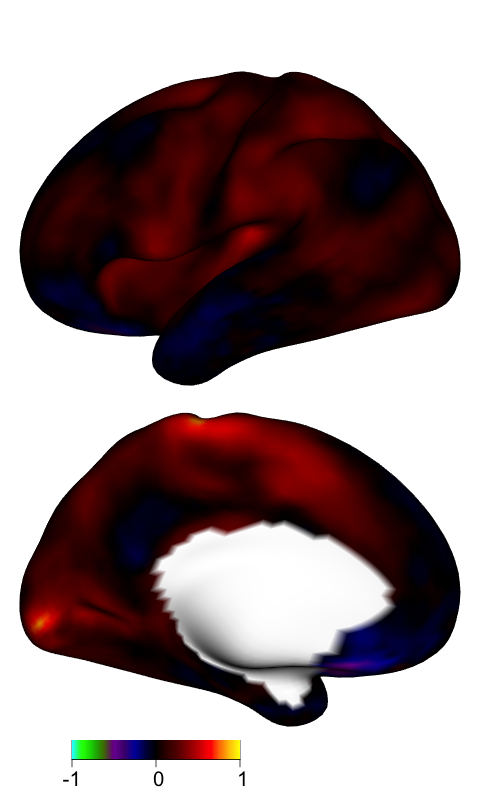
\includegraphics[width=0.2\textwidth]{plots/601_group_Bayes_right_hand.png} \\ \hline
%				\rotatebox{90}{\textbf{Classical GLM}} & 
%				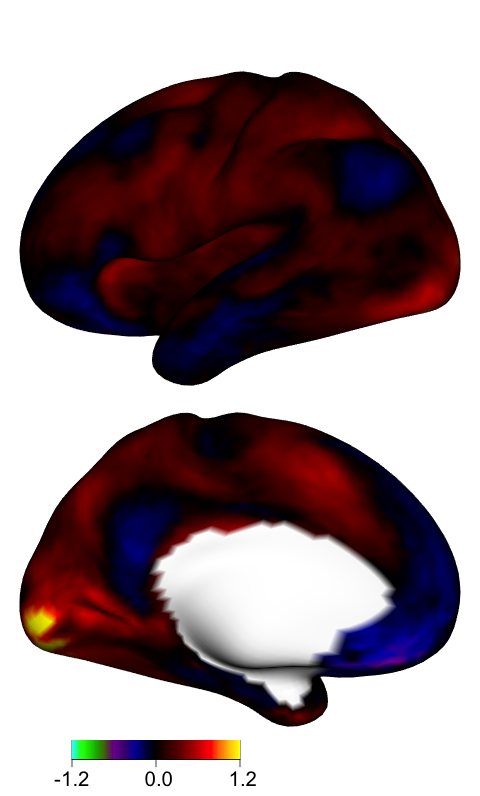
\includegraphics[width=0.2\textwidth]{plots/601_group_classical_visual_cue.png} &
%				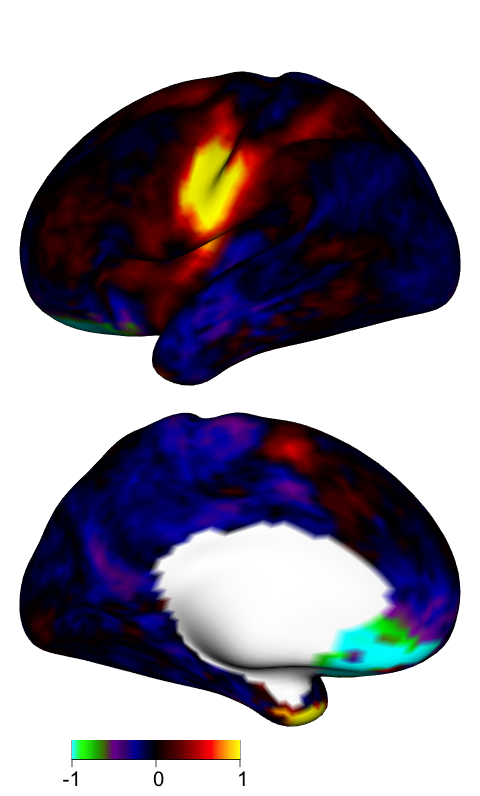
\includegraphics[width=0.2\textwidth]{plots/601_group_classical_tongue.png} &
%				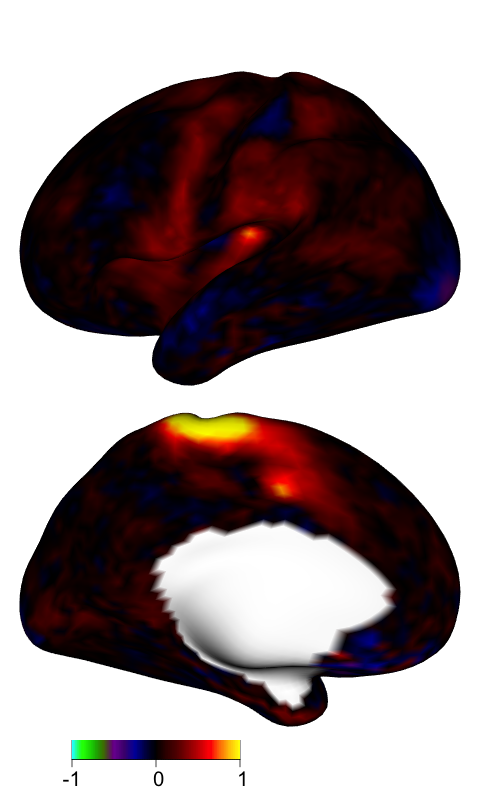
\includegraphics[width=0.2\textwidth]{plots/601_group_classical_right_foot.png} &
%				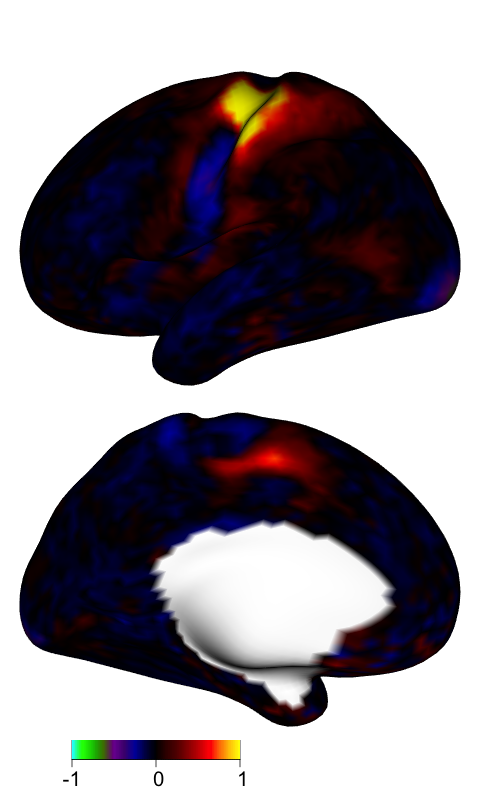
\includegraphics[width=0.2\textwidth]{plots/601_group_classical_right_hand.png} \\ \hline
%			\end{tabularx}
%		\caption{Estimates of activation amplitude in terms of percent signal change.}
%		\label{subfig:group_est}
%		\end{subfigure}
%	
%		\begin{subfigure}{\textwidth}
%			\begin{tabularx}{\textwidth}{|m{1em}|X|X|X|X|}
%				\hline
%				\rotatebox{90}{\textbf{Bayesian GLM}}& 
%				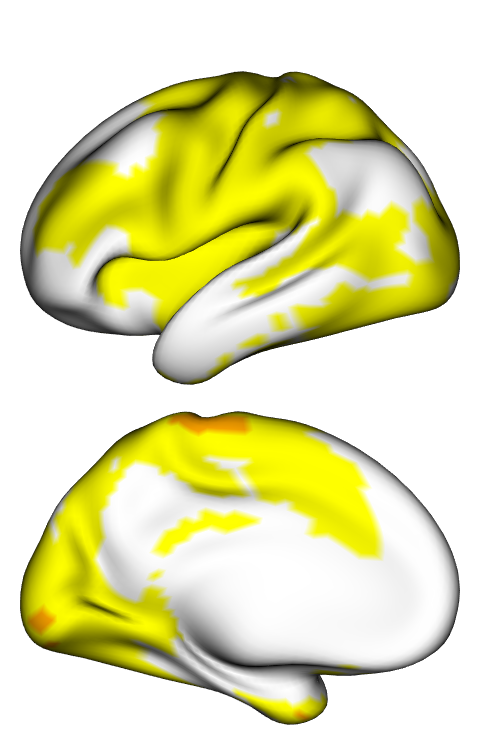
\includegraphics[width=0.2\textwidth]{plots/603_visual_cue_activation_map.png} &
%				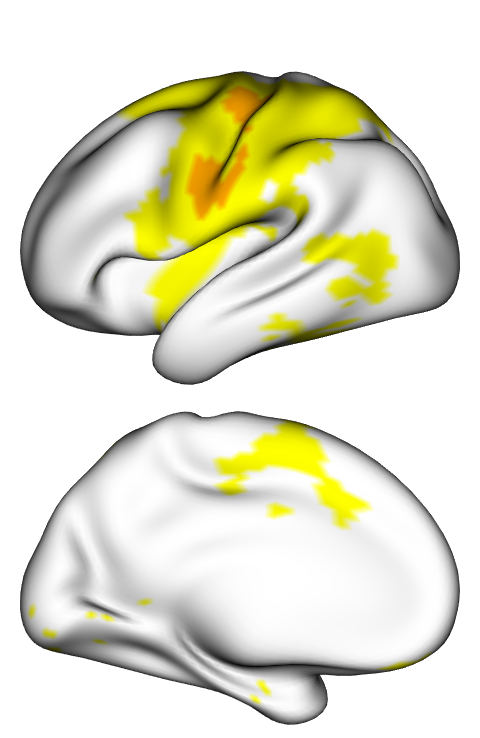
\includegraphics[width=0.2\textwidth]{plots/603_tongue_activation_map.png} &
%				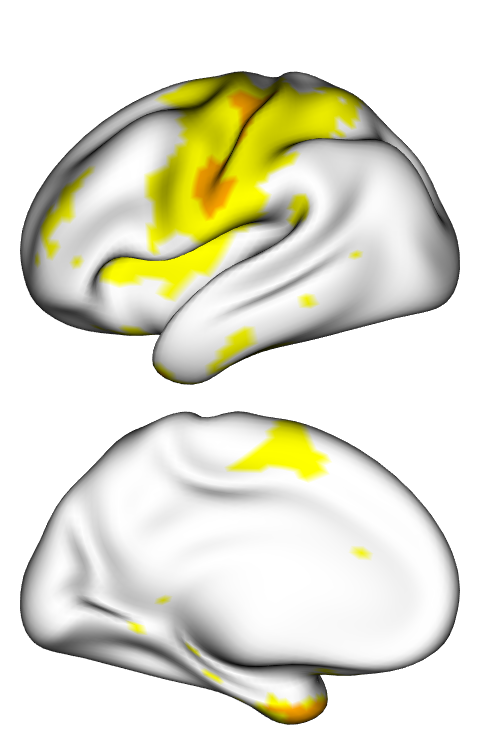
\includegraphics[width=0.2\textwidth]{plots/603_foot_activation_map.png} &
%				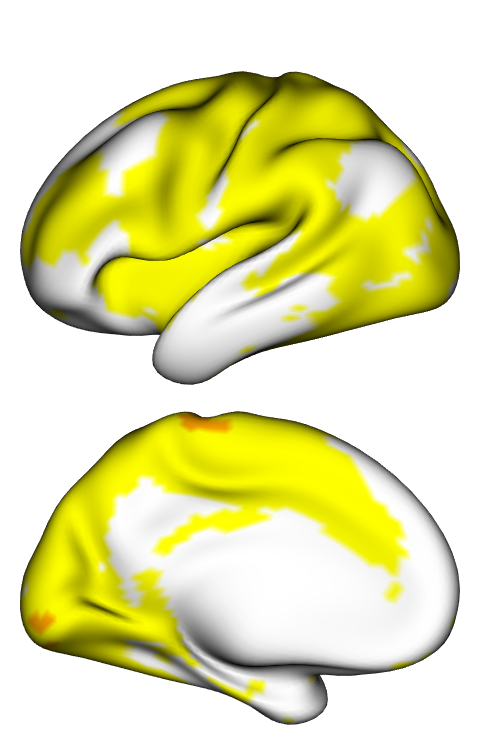
\includegraphics[width=0.2\textwidth]{plots/603_hand_activation_map.png} \\ \hline
%				\multicolumn{2}{c}{} & \multicolumn{2}{c}{$\gamma = $ \textcolor{yellow}{$\blacksquare$} $0\%$ \textcolor{orange}{$\blacksquare$} $0.5\%$ } & \multicolumn{1}{c}{} \\ \hline
%				\rotatebox{90}{\textbf{Classical GLM}} & 
%				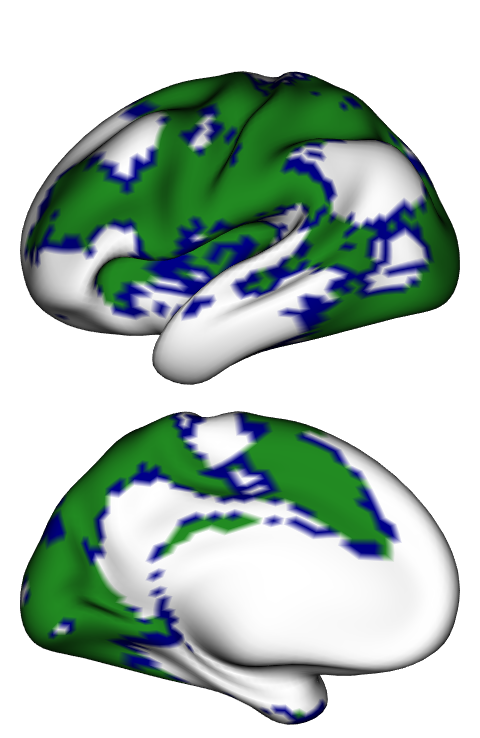
\includegraphics[width=0.2\textwidth]{plots/604_visual_cue_classical_activation_map.png} &
%				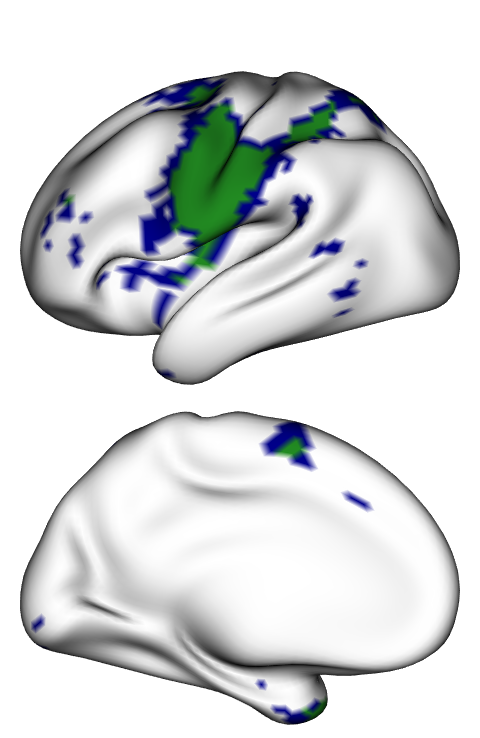
\includegraphics[width=0.2\textwidth]{plots/604_tongue_classical_activation_map.png} &
%				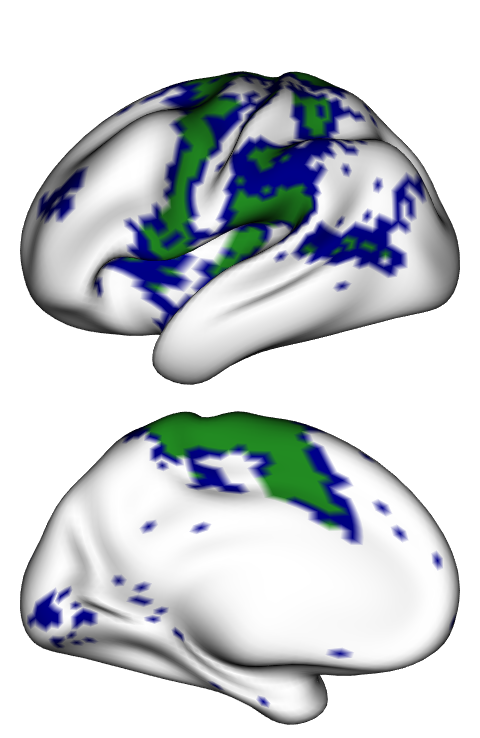
\includegraphics[width=0.2\textwidth]{plots/604_foot_classical_activation_map.png} &
%				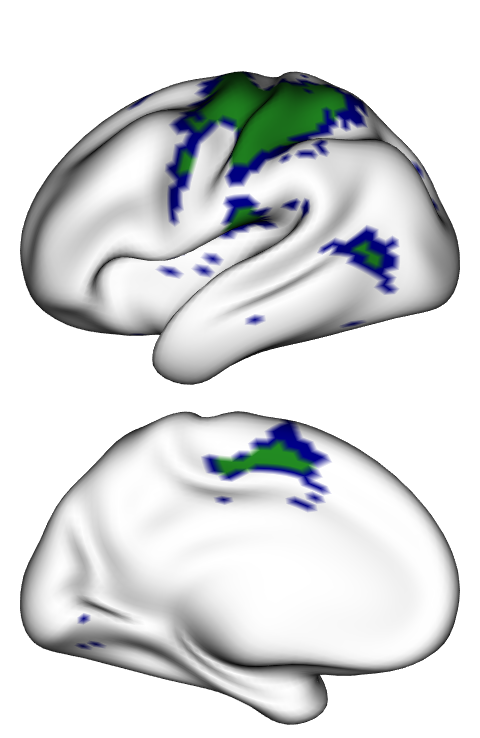
\includegraphics[width=0.2\textwidth]{plots/604_hand_classical_activation_map.png} \\ \hline
%				\multicolumn{2}{c}{} & \multicolumn{2}{c}{\textcolor{Blue}{$\blacksquare$} FDR \textcolor{OliveGreen}{$\blacksquare$} FWER } & \multicolumn{1}{c}{} \\
%			\end{tabularx}	
%		\caption{Areas of activations based on the significance level $\alpha = 0.01$.}
%		\label{subfig:group_act}
%		\end{subfigure}
%	\caption{Group-level estimates of activation amplitude (\ref{subfig:group_est}) and areas of activation (\ref{subfig:group_act}) for four tasks of the motor study. For the Bayesian GLM, the estimates displayed are group-level posterior means, and the areas of activation are based on two different activation thresholds $\gamma$ (0\% and 0.5\% local signal change.)}
%	\label{fig:group_est_and_act}
%	\end{figure}

%	\newpage
%	
%	\pagestyle{empty}
%	
%		\begin{figure}
%		\begin{subfigure}{\textwidth}
%			\begin{tabularx}{\textwidth}{|m{1em}|X|X|}
%				\multicolumn{1}{c}{} & \multicolumn{1}{c}{\textbf{Single Subject}} & \multicolumn{1}{c}{\textbf{Group Analysis}}  \\ \hline
%				\rotatebox{90}{\textbf{Bayesian GLM}}& 
%				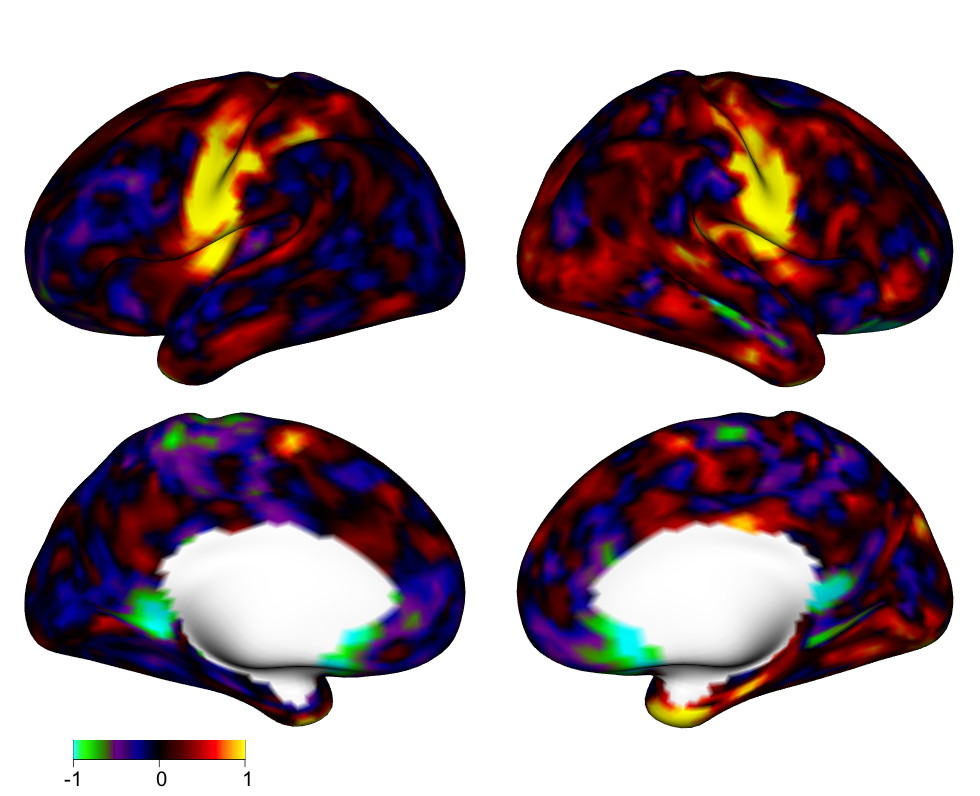
\includegraphics[width=0.4\textwidth]{plots/601_subject_bayes_tongue_estimate.png} &
%				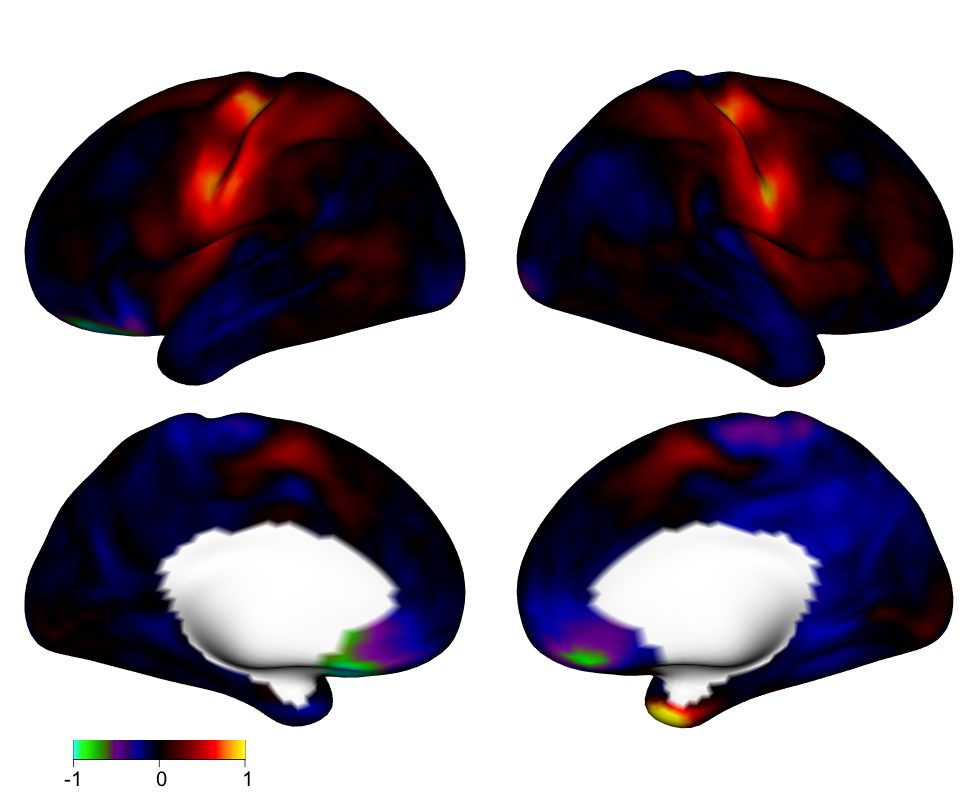
\includegraphics[width=0.4\textwidth]{plots/601_group_bayes_tongue_estimate.png} \\ \hline
%				\rotatebox{90}{\textbf{Classical GLM}} & 
%				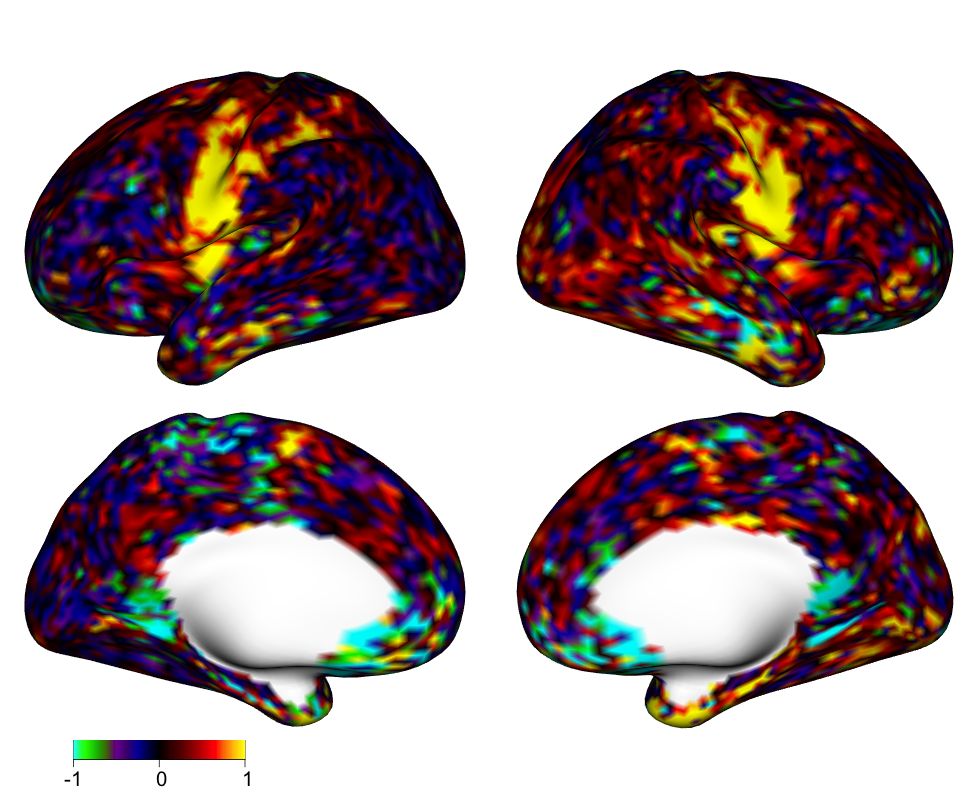
\includegraphics[width=0.4\textwidth]{plots/601_subject_classical_tongue_estimate.png} &
%				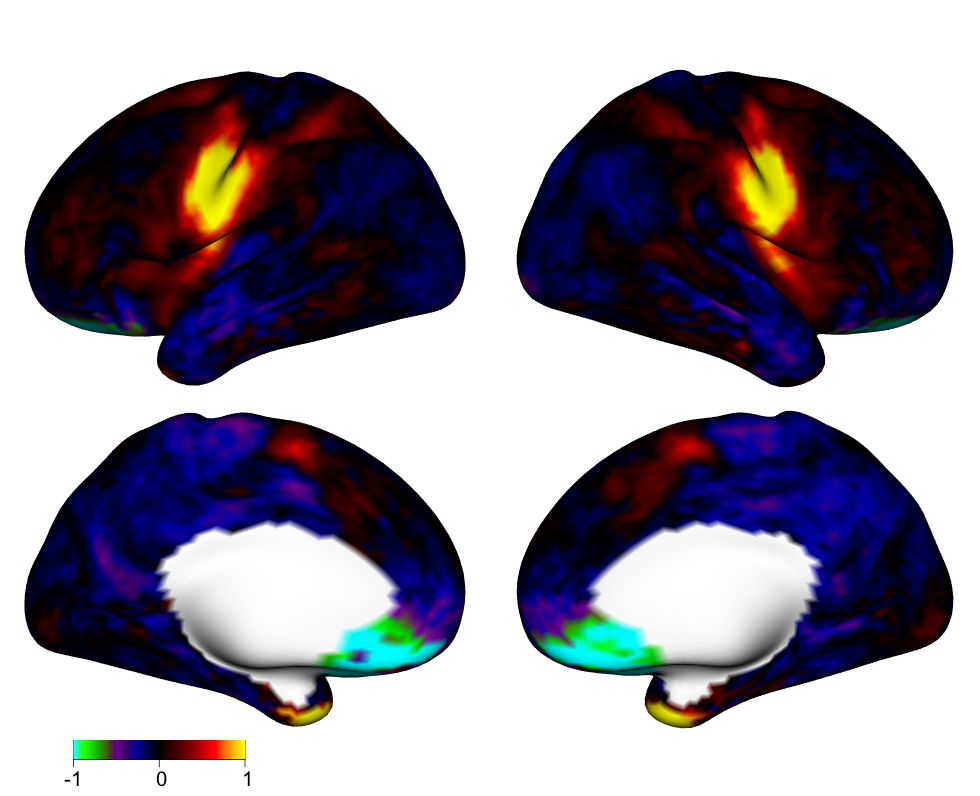
\includegraphics[width=0.4\textwidth]{plots/601_group_classical_tongue_estimate.png}  \\ \hline
%			\end{tabularx}
%			\caption{Estimates of activation amplitude in terms of percent signal change.}
%			\label{subfig:tongue_est}
%		\end{subfigure}
%		
%		\begin{subfigure}{\textwidth}
%			\begin{tabularx}{\textwidth}{|m{1em}|X|X|}
%				\multicolumn{1}{c}{} & \multicolumn{1}{c}{\textbf{Single Subject}} & \multicolumn{1}{c}{\textbf{Group Analysis}}  \\ \hline
%				\rotatebox{90}{\textbf{Bayesian GLM}}& 
%				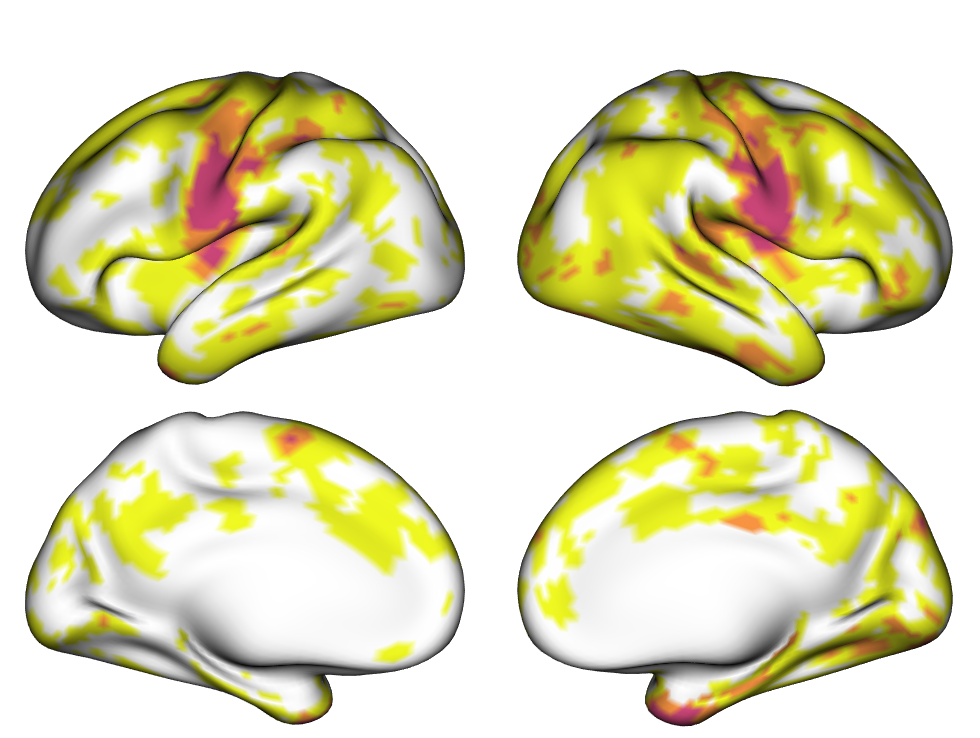
\includegraphics[width=0.4\textwidth]{plots/601_subject_bayes_tongue_activation.png} &
%				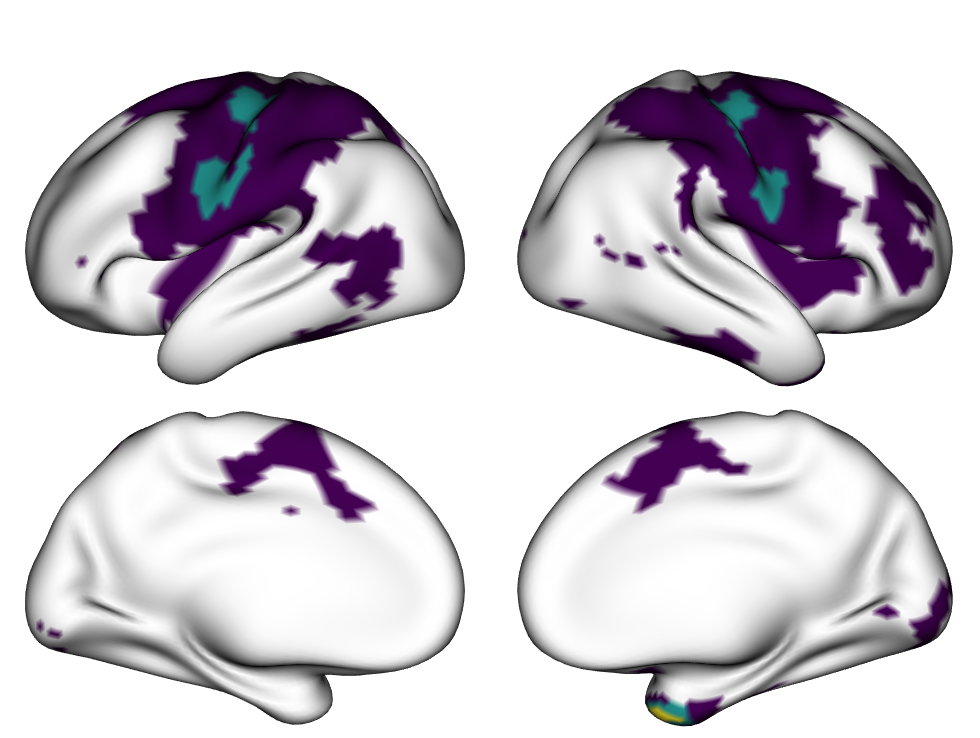
\includegraphics[width=0.4\textwidth]{plots/601_group_bayes_tongue_activation.png} \\ 
%				\hline
%				\multicolumn{1}{c}{} & \multicolumn{2}{c}{$\gamma = $ \textcolor[HTML]{440154}{$\blacksquare$} $0\%$ \textcolor[HTML]{21908C}{$\blacksquare$} $0.5\%$ \textcolor[HTML]{FDE725}{$\blacksquare$} $1\%$}  \\ \hline
%				\rotatebox{90}{\textbf{Classical GLM}} & 
%				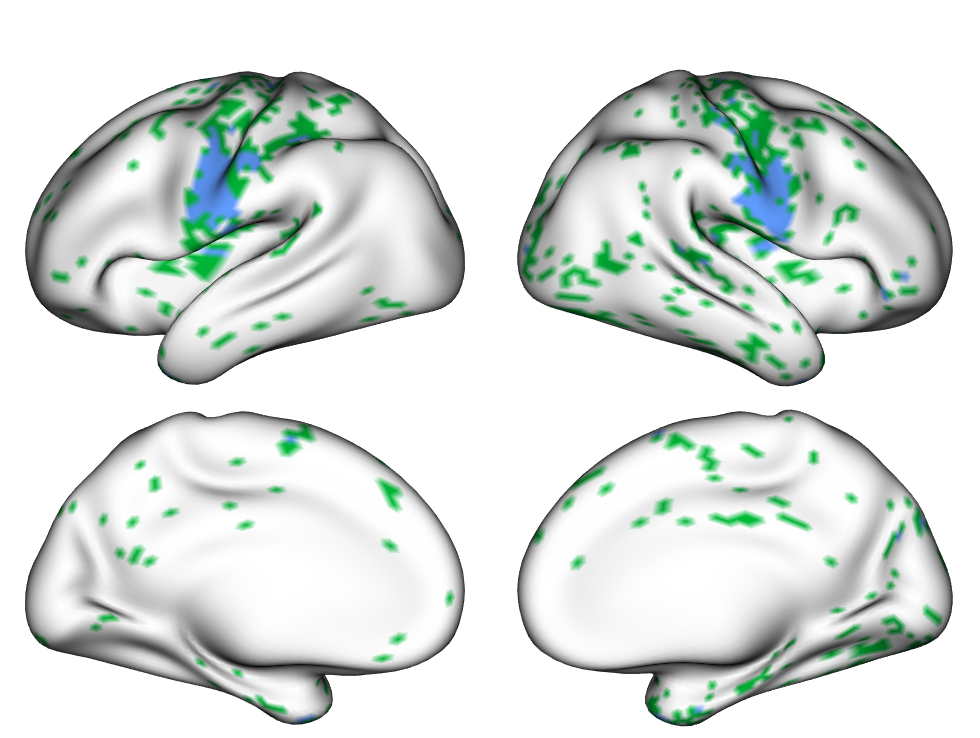
\includegraphics[width=0.4\textwidth]{plots/601_subject_classical_tongue_activation.png} &
%				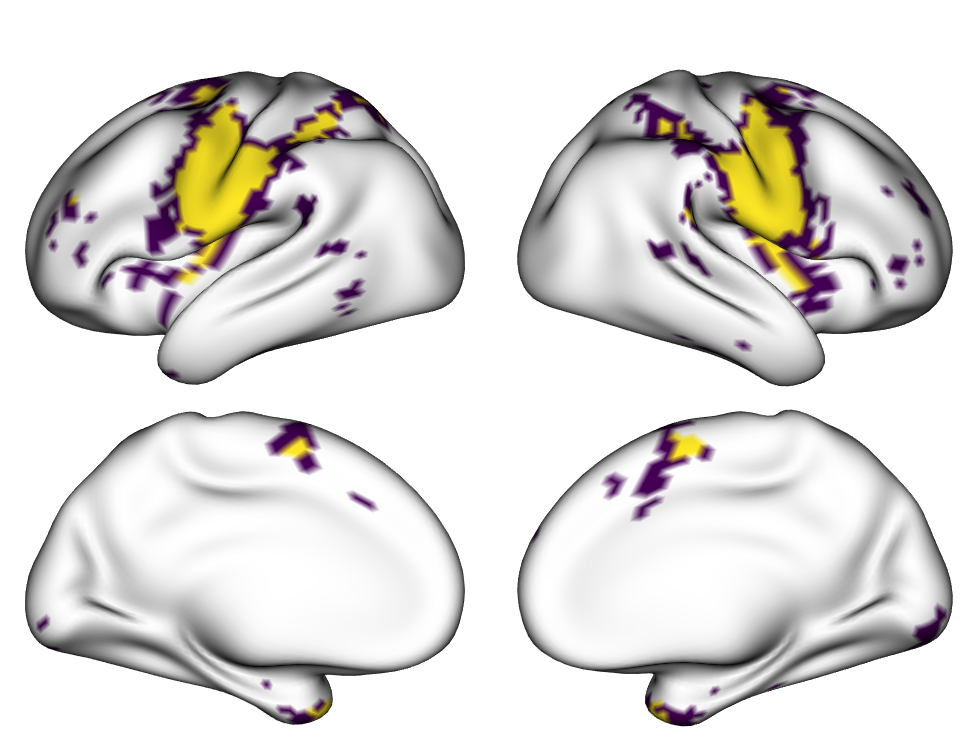
\includegraphics[width=0.4\textwidth]{plots/601_group_classical_tongue_activation.png}  \\ 
%				\hline
%				\multicolumn{1}{c}{} & \multicolumn{2}{c}{\textcolor[HTML]{440154}{$\blacksquare$} FDR \textcolor[HTML]{FDE725}{$\blacksquare$} FWER } \\
%			\end{tabularx}
%			\caption{Estimates of activation amplitude in terms of percent signal change.}
%			\label{subfig:tongue_act}
%		\end{subfigure}
%		\caption{ Single-subject and group-level estimates of activation amplitude (\ref{subfig:tongue_est}) and areas of activation (\ref{subfig:tongue_act}) for both brain hemispheres for the tongue task. For the Bayesian GLM, the estimates displayed are group-level posterior means, and the areas of activation are based on three different activation thresholds $\gamma$ (0\%, 0.5\%, and 1\% local signal change.)}
%		\label{fig:tongue_est_and_act}
%	\end{figure}

\newpage

\pagestyle{empty}

\begin{figure}
		\begin{tabularx}{\textwidth}{|X|X|}
			\multicolumn{1}{c}{\textbf{Classical GLM}} & \multicolumn{1}{c}{\textbf{Bayesian GLM}}  \\ \hline
			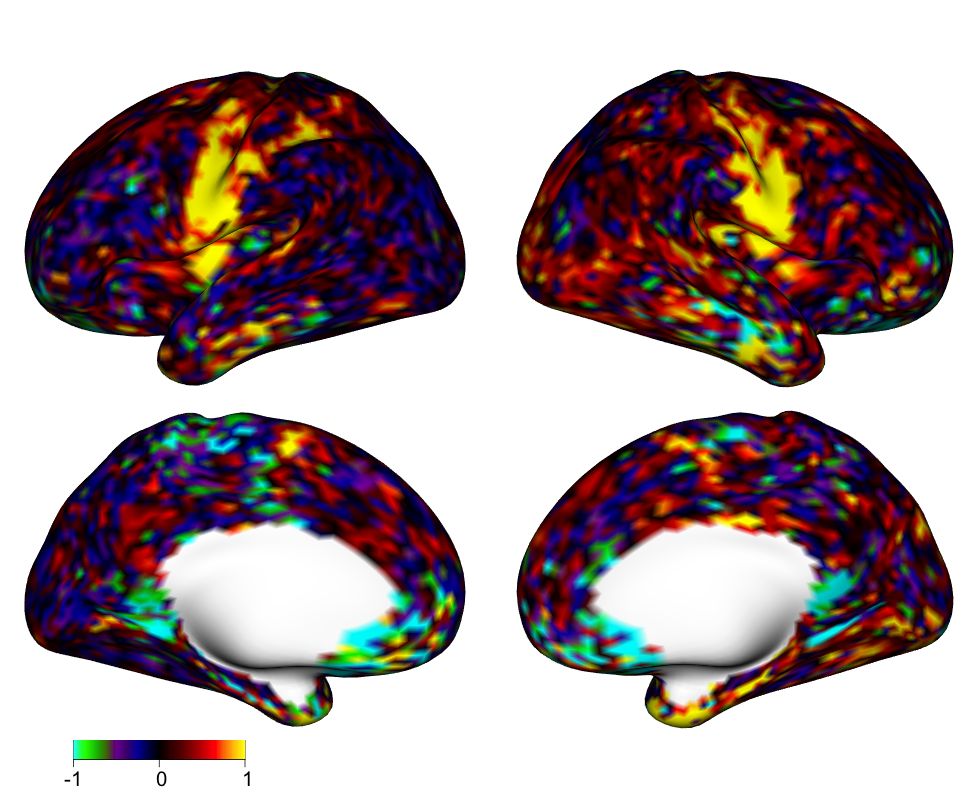
\includegraphics[width=0.48\textwidth]{plots/601_subject_classical_tongue_estimate.png} &
			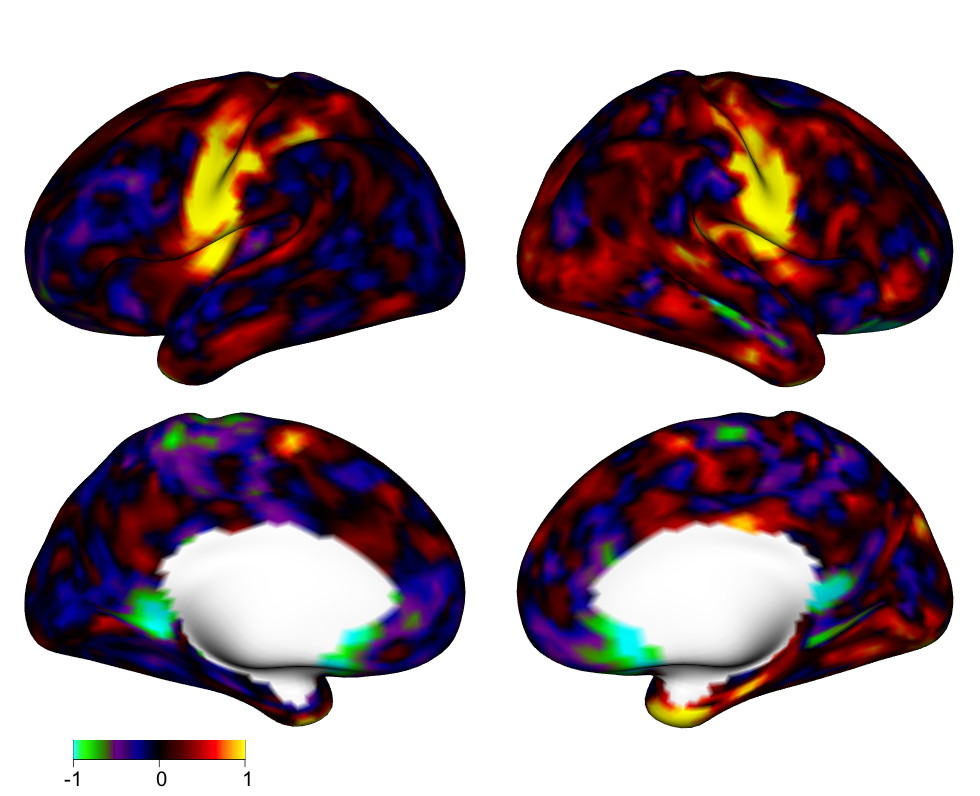
\includegraphics[width=0.48\textwidth]{plots/601_subject_bayes_tongue_estimate.png} \\ \hline
			\includegraphics[width=0.48\textwidth]{plots/601_subject_classical_tongue_activation.png} &
			\includegraphics[width=0.48\textwidth]{plots/601_subject_bayes_tongue_activation.png}  \\ 
			\multicolumn{1}{|c|}{\textcolor[HTML]{00BA38}{$\blacksquare$} FDR \textcolor[HTML]{619CFF}{$\blacksquare$} FWER } &
			\multicolumn{1}{c|}{$\gamma = $ \textcolor[HTML]{F0F921}{$\blacksquare$} $0\%$ \textcolor[HTML]{F89441}{$\blacksquare$} $0.5\%$ \textcolor[HTML]{CC4678}{$\blacksquare$} $1\%$}\\
			\hline
		\end{tabularx}
	\caption{Single-subject estimates of activation amplitude and areas of activation for both brain hemispheres for the tongue task. For the classical GLM, areas of activation are found using the FDR and FWER multiple testing corrections. For the Bayesian GLM, the areas of activation are based on three different activation thresholds $\gamma$ (0\%, 0.5\%, and 1\% local signal change). All activations were determined using a one-sided significance level of 0.01.}
	\label{fig:tongue_est_and_act}
\end{figure}
	
	\newpage

	\section{Intraclass Correlation}
	
%	\begin{figure}
%		\begin{tabularx}{\textwidth}{|X|X|}
%			\hline
%%			\rotatebox{90}{\textbf{Bayesian GLM}}& 
%			\includegraphics[width=0.48\textwidth]{plots/601_subject_bayes_tongue_icc.png} &
%			\includegraphics[width=0.48\textwidth]{plots/601_wicc_plot.png} \\ \hline
%%			\rotatebox{90}{\textbf{Classical GLM}} & 
%			\includegraphics[width=0.48\textwidth]{plots/601_subject_classical_tongue_icc.png} &
%			\includegraphics[width=0.48\textwidth]{plots/601_dice_plot.png} \\ \hline
%		\end{tabularx}	
%		\caption{Cross-subject average intraclass correlation coefficient (ICC) values for the similarity of average amplitude estimates across the two visits in the study data for the tongue motor task for the Bayesian GLM and the Classical GLM (left panels). The weighted ICC summary statistic (top right) and boxplots for the Dice coefficient for each subject (bottom right) across the two models is shown for all four tasks.}
%		\label{fig:icc}
%	\end{figure}

\begin{figure}
	\begin{tabularx}{\textwidth}{|X|X|}
		\hline
		%			\rotatebox{90}{\textbf{Bayesian GLM}}& 
		\includegraphics[width=0.48\textwidth]{plots/601_subject_classical_tongue_icc.png} &
		\includegraphics[width=0.48\textwidth]{plots/601_subject_bayes_tongue_icc.png} \\ \hline
		%			\rotatebox{90}{\textbf{Classical GLM}} & 
		\multicolumn{2}{c}{\includegraphics[width=0.96\textwidth]{plots/601_wicc_plot.png}} \\
		\multicolumn{2}{c}{\includegraphics[width=0.96\textwidth]{plots/601_dice_plot.png}} \\ \hline
	\end{tabularx}	
	\caption{Cross-subject average intraclass correlation coefficient (ICC) values for the similarity of average amplitude estimates across the two visits in the study data for the tongue motor task for the Classical GLM and the Bayesian GLM (top panels). The weighted ICC summary statistic with weights based on the group classical GLM activation (middle panel) and boxplots for the Dice coefficient for each subject (bottom panel) across the two models is shown for all six tasks.}
	\label{fig:icc}
\end{figure}

\end{document}